\section{Observation and Calculation}
	\subsection{Transistor charecteristics}
		\begin{figure}[h]
			\centering
			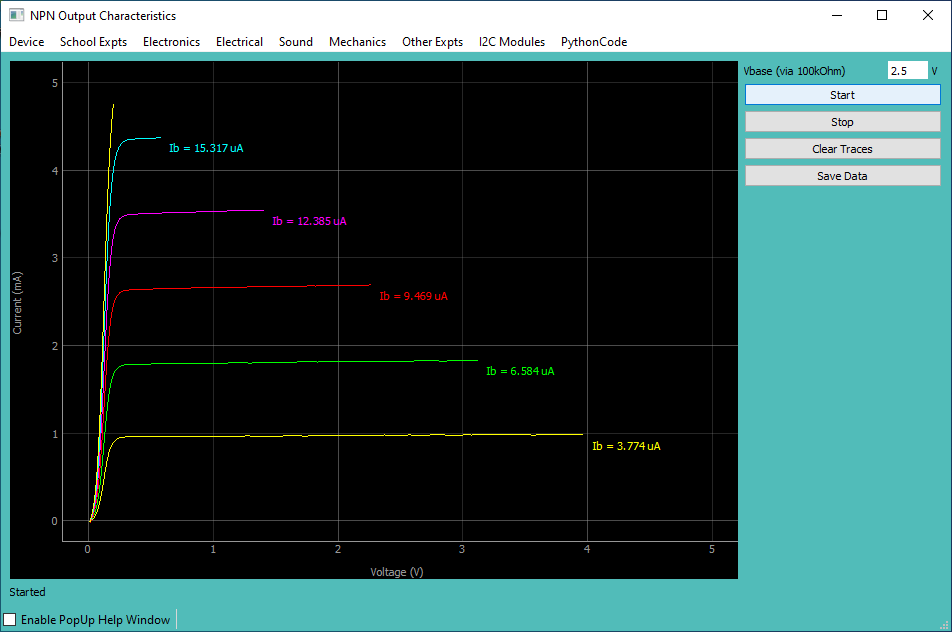
\includegraphics[width=0.8\columnwidth]{images/tc.png}
			\caption{Transistor charecterictics}
			\label{ss:1}
		\end{figure}
		The transistor characteristics for the given NPN transistor is shown \hyperref[ss:1]{Figure 5}.

	\subsection{Astable multivibrator with IC 555}
		\begin{figure}[h]
			\centering
			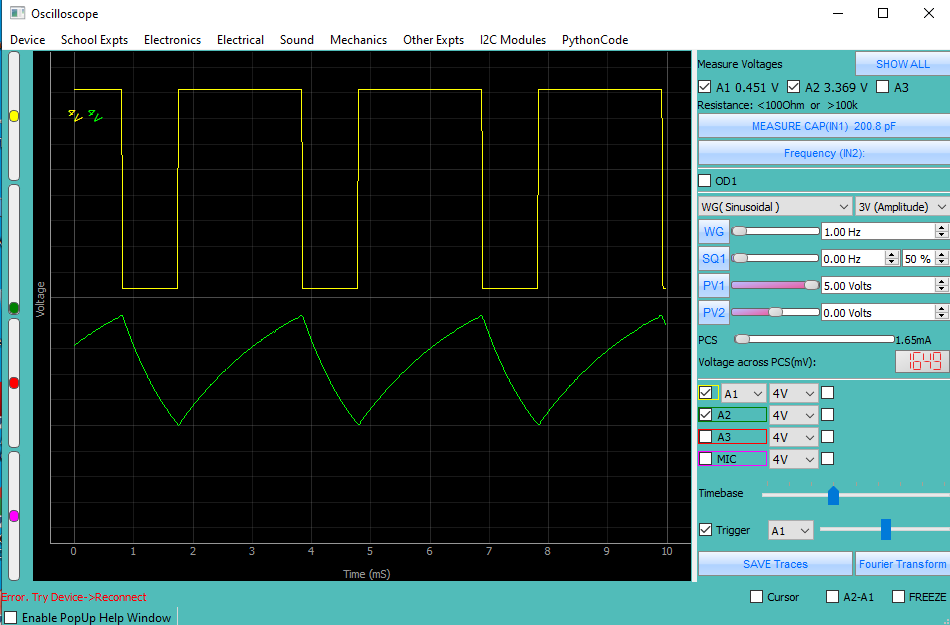
\includegraphics[width=0.8\columnwidth]{images/dc100.png}
			\caption{voltage vs time graph for Astable multivibrator with duty cycle less than $50\%$}
			\label{ss:2}
		\end{figure}

		theoretically, $f=720Hz$, Duty cycle=$50\%$

		observed, $f=476.19Hz$,
		
		$$\text{Duty cycle}=\frac{T_1}{T_1+T_2}=67\%$$

		\begin{figure}[h]
			\centering
			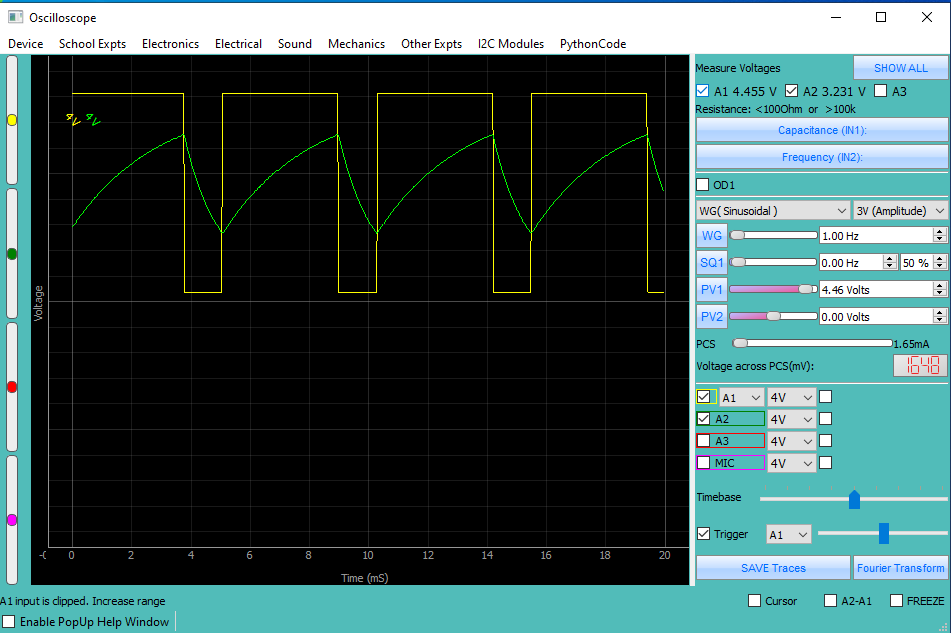
\includegraphics[width=0.8\columnwidth]{images/dc50.png}
			\caption{ voltage vs time graph for Astable multivibrator with duty cycle more than $50\%$}
			\label{ss:3}
		\end{figure}

		theoretically, f=389.1Hz, Duty cycle=$72.9\%$

		observed, f=381Hz,
		
		$$\text{Duty cycle}=\frac{T_1}{T_1+T_2}=80\%$$

	\subsection{EM induction}
		
		\begin{figure}[h]
			\centering
			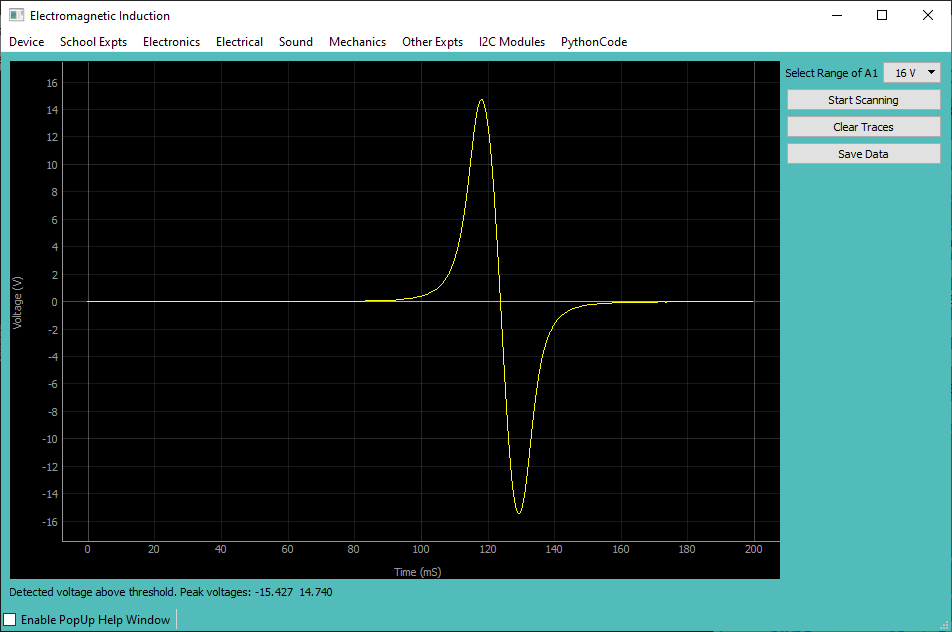
\includegraphics[width=0.8\columnwidth]{images/emf.png}
			\caption{Emf versus time graph for a vertically dropping magnet}
			\label{ss:4}
		\end{figure}

		From \hyperref[eq:4]{Equation 4} we have

		We know that: $z_o=\frac{\text{length of coil}}{2} = 0.01 m$

		Also given:
		$N=3000$
		$t = 115 ms$
		$emf = 14.740V$
		$R = 0.002 m$

		Thus, $m=0.2161Am^2$
